\chapter{Sensing and estimation}
\label{chap:estimation}
\chaptermark{Sensing and estimations}

The wake model discussed in Chapter~\ref{chap:dynwake} includes important aspects of wake advection, expansion, and interaction that have significant effects on the total wind farm power production. However, the model makes a number of simplifying assumptions, such as linear advection and neglecting spanwise wake interactions, and neglects natural variations in power production due to turbulence within the wind farm. There is also uncertainty in the model parameters, specifically the freestream velocity $U_\infty$ and the wake expansion coefficients $k_n$. 

Measurements that are readily available in existing wind farms may be able to correct many of these modeling errors. In addition to measurements of the power production at each turbine, velocity field and wind heading information can be obtained from a wide range of sensors. Sonic and propeller anemometers and wind vanes provide point source measurements of velocity~\cite{Pao2011a}, blade loads can be used to estimate wind alignment, wind shear, and wake locations~\cite{Bottasso2014a, Bottasso2018a}, and lidar measurements can be used to track wake positions~\cite{Raach2016a, Churchfield2016a}. Various measurements also can be combined to make estimates of other quantities such as the effective rotor-averaged wind speed~\cite{Knudsen2011a}.

All of the control designs considered in this thesis use power measurements for closed loop feedback. We consider two approaches that differ significantly in complexity. First, we consider a temporally damped correction term in Section~\ref{sec:estimation-damped} that does not directly correct model states or parameters. Instead, it provides a means of adjusting the current model output equation to improve the model based receding horizon control of Chapter~\ref{chap:rhc}. Second, we consider an ensemble based state and parameter estimation method in Section~\ref{subsec:estimation-ensemble-enkf}. At the cost of additional complexity, this approach provides online estimation of model parameters as well as direct state corrections to improve the model predictions.

\section{Temporally damped correction}
\label{sec:estimation-damped}
The simplest feedback used is a temporally-damped error correction term for the modeled rotor-averaged axial velocity. From the measured power production of the $m$-th turbine in the $n$-th row, the row-averaged power and row- and rotor-averaged wind velocities are defined as
\begin{equation}
\qquad P_n = \sum_{m=1}^M P_{nm}, \quad \text{and} \qquad \qquad u_n = \frac{1}{M}\left(   \sum_{m=1}^M u_{nm}^3  \right)^{1/3},
\end{equation}
where $u_{nm}$  is the velocity measured at the turbine in the $n$-th row and $m$-th column of the wind farm. The definition of the row-average velocity at the turbine disk is necessary to ensure that  the expression for the turbine output power $P_n = M \frac{1}{2} \rho \frac{\pi D^2}{4} C_{Tn}' u_{n}^3$ is satisfied. These measurements are used to calculate an error term $\epsilon_n$ and provide feedback by replacing Eq.~\eqref{eq:estimated_power_row} with
\begin{equation}
\hat{P}_n = M \frac{1}{2}\rho \frac{\pi D^2}{4} C_{Tn}' (\hat{u}_n + \epsilon_n)^3.
\end{equation}
The error correction at the current time $t_c$ is 
\begin{equation}
\epsilon_n(t) = \left(u_n(t_c) -  \hat{u}_n (t_c) \right) e^{-(t-t_c)/\tau}.
\end{equation}
The exponential decay accounts for the reduced  future accuracy of the error term in the prediction and is set to $\tau = 120$ s in the applicable results in Chapter~\ref{chap:rhc}.

While this feedback correction is simple to implement and incorporates the diminishing utility of  measurements further in the future, there are several deficiencies with this approach. First, the method assumes that the current measurement is perfectly accurate and ignores measurement error. Second, the corrections only affect the predictions at the turbine at which the measurement is taken. In the advective atmospheric boundary layer, past measurements at upstream turbines should affect the current estimate at downstream turbines. Finally, this method does not estimate the wake model parameters, which must be calculated in another way.

\section{Ensemble-based optimal estimation}
\label{sec:estimation-ensemble}

The second error correction method used is an ensemble based state and parameter estimation method employing an ensemble Kalman filter (EnKF)~\cite{Evensen2003a}. This approach provides online estimation of model parameters as well as state estimates. The EnKF approaches the properties of the standard Kalman filter (KF), but at significant computational savings. In this section, we first describe the canonical KF in Section~\ref{subsec:estimation-ensemble-kalman}. We then describe in Section~\ref{subsec:estimation-ensemble-enkf} the EnKF's approximation of the KF's error covariance matrix using an ensemble of state space representations and the associated forecast and analysis equations. Finally, we describe the details of the state and parameter estimation for the wake model of Section~\ref{sec:dynwake-1d} in Section~\ref{subsec:estimation-ensemble-wake} and validate the results using LES in Section~\ref{subsec:estimation-ensemble-validation}.

\subsection{The Kalman filter}
\label{subsec:estimation-ensemble-kalman}

The Kalman filter is a celebrated accomplishment of modern control theory that provides a rigorous method for estimating the state of a linear system using measurements and knowledge of the system's properties~\cite{Kalman1960a, Gelb1974a}. President Obama noted the profound impact of the Kalman filter upon awarding Rudolf Kalman the 2008 National Medal of Science 

\begin{quote}
for his invention of the ``Kalman filter," which was critical to achieving the Moon landings and creating the Global Positioning System and which has facilitated the use of computers in control and communications technology.~\cite{Obama2009a}
\end{quote}

In this thesis, we will follow the Kalman filter derivation of Gelb \textit{et al.}~\cite{Gelb1974a}. We consider linear, discrete-time, possibly time-varying system of equations between time steps $k$ and $k+1$ 
\begin{align}
\label{eq:linear_plant1}
\boldsymbol{\psi}_{k+1} &= \mathbf{A}_k \boldsymbol{\psi}_k + \mathbf{B}_k \boldsymbol{\gamma}_k + \mathbf{J}_k\boldsymbol{\chi}_k \\
\label{eq:linear_plant2}
\boldsymbol{\xi}_k &= \mathbf{C}_k\boldsymbol{\psi}_k + \mathbf{D}_k\boldsymbol{\gamma}_k + \boldsymbol{\epsilon}_k.
\end{align}
The matrices $\mathbf{A}_k \in \mathbb{R}^{N_s \times N_s}$, $\mathbf{B}_k \in \mathbb{R}^{N_s \times N_i}$, $\mathbf{J}_k \in \mathbb{R}^{N_s \times N_p}$, $\mathbf{C}_k \in \mathbb{R}^{N_m \times N_s}$, $\mathbf{D}_k \in \mathbb{R}^{N_m \times N_i}$ are known from the physics of the problem. The state variables are $\boldsymbol{\psi} \in \mathbb{R}^{N_s}$, the measurement variables are $\boldsymbol{\xi} \in \mathbb{R}^{N_m}$ and the deterministic and known input variables are $\boldsymbol{\gamma} \in \mathbb{R}^{N_i}$. The white process noise $\boldsymbol{\chi} \in \mathbb{R}^{N_p}$ and measurement noise $\boldsymbol{\epsilon} \in \mathbb{R}^{N_m}$ both have zero mean and known covariances
\begin{align}
\mathrm{E}[\boldsymbol{\chi}_k \boldsymbol{\chi}_k^T] &= \mathbf{Q}_k \qquad \qquad& \mathrm{E}[\boldsymbol{\chi}_k] &= \mathbf{0} \\
\mathrm{E}[\boldsymbol{\epsilon}_k \boldsymbol{\epsilon}_k^T] &= \mathbf{R}_k \qquad \qquad & \mathrm{E}[\boldsymbol{\epsilon}_k] &= \mathbf{0},
\end{align}
where $\mathrm{E}[\cdot]$ denotes an expectation. 

Given knowledge of the measurements $\boldsymbol{\xi}$ and the inputs $\boldsymbol{\gamma}$, the Kalman filter seeks a minimum-variance estimate of the states of the system $\bar{\boldsymbol{\psi}}$. The discrete-time Kalman filter is a recursive filter that begins with an initial estimate of the states $\bar{\boldsymbol{\psi}}_k$ at time $k$ and does not require storage of past estimates or measurements. The state estimate is first forecasted using an \textit{a priori} estimate, denoted as step $k+$, from the current state
\begin{align}
\label{eq:linear_forecast1}
\bar{\boldsymbol{\psi}}_{k+} &= \mathbf{A}_k \bar{\boldsymbol{\psi}}_k + \mathbf{B}_k \boldsymbol{\gamma}_k \\
\label{eq:linear_forecast2}
\bar{\boldsymbol{\xi}}_{k+} &= \mathbf{C}_k\bar{\boldsymbol{\psi}}_{k+} + \mathbf{D}_k\boldsymbol{\gamma}_k.
\end{align}
The subsequent analysis step is an \textit{a posteriori} update using measurements from the system 
\begin{align}
\label{eq:linear_analysis1}
\bar{\boldsymbol{\psi}}_{k+1} &= \bar{\boldsymbol{\psi}}_{k+} + \mathbf{K}_k(\boldsymbol{\xi}_k - \bar{\boldsymbol{\xi}}_{k+}) \\
\label{eq:linear_analysis2}
\bar{\boldsymbol{\xi}}_{k+1} &= \mathbf{C}_{k+1}\bar{\boldsymbol{\psi}}_{k+1} + \mathbf{D}_{k+1}\boldsymbol{\gamma}_{k+1},
\end{align}
where $\mathbf{K}_k$ is the currently unknown Kalman gain matrix that must be determined.

The state error $\boldsymbol{e}_k = \boldsymbol{\psi}_k - \bar{\boldsymbol{\psi}}_k$ at the previous time step can be used to recursively find the state error of the forecast
\begin{equation}
\begin{split}
\boldsymbol{e}_{k+} &= \boldsymbol{\psi}_{k+1} - \bar{\boldsymbol{\psi}}_{k+}\\
&= \mathbf{A}_k \boldsymbol{\psi}_k + \mathbf{B}_k \boldsymbol{\gamma}_k + \mathbf{J}_k\boldsymbol{\chi}_k - \left(\mathbf{A}_k \bar{\boldsymbol{\psi}}_k + \mathbf{B}_k \boldsymbol{\gamma}_k\right)\\
&= \mathbf{A}_k \boldsymbol{e}_k + \mathbf{J}_k\boldsymbol{\chi}_k
\end{split}
\end{equation}
and analysis steps
\begin{equation}
\begin{split}
\boldsymbol{e}_{k+1} &= \boldsymbol{\psi}_{k+1} - \bar{\boldsymbol{\psi}}_{k+1}\\
&= \boldsymbol{\psi}_{k+1} - \bar{\boldsymbol{\psi}}_k - \mathbf{K}_k(\mathbf{C}_k\boldsymbol{\psi}_k + \mathbf{D}_k\boldsymbol{\gamma}_k + \boldsymbol{\epsilon}_k -  \mathbf{C}_k\bar{\boldsymbol{\psi}}_{k+} - \mathbf{D}_k\boldsymbol{\gamma}_k )\\
&= (\mathbf{I} - \mathbf{K}_k\mathbf{C}_k) \boldsymbol{e}_{k+} + \mathbf{K}_k \boldsymbol{\epsilon}_k.
\end{split}
\end{equation}
From these state error definitions, we can define error covariance matrices for the forecast step
\begin{equation}
\begin{split}
\mathbf{P}_{k+} &= E\left[ \boldsymbol{e}_{k+} \boldsymbol{e}_{k+}^T \right] \\
&= \mathbf{A}_k \mathrm{E}[\boldsymbol{e}_k  \boldsymbol{e}_k^T]\mathbf{A}_k^T + \mathbf{J}_k \mathrm{E}[\boldsymbol{\chi}_k  \boldsymbol{\chi}_k^T]\mathbf{J}_k^T \\
&= \mathbf{A}_k \mathbf{P}_k \mathbf{A}_k^T + \mathbf{J}_k  \mathbf{Q}_k \mathbf{J}_k^T 
\end{split}
\end{equation}
and analysis step
\begin{equation}
\begin{split}
\mathbf{P}_{k+1} &= \mathrm{E} \left[ \boldsymbol{e}_{k+1} \boldsymbol{e}_{k+1}^T \right] \\
&=  (\mathbf{I} - \mathbf{K}_k\mathbf{C}_k) \mathrm{E}[\boldsymbol{e}_{k+} \boldsymbol{e}_{k+}^T]  (\mathbf{I} - \mathbf{K}_k\mathbf{C}_k)^T + \mathbf{K}_k \mathrm{E}[\boldsymbol{\epsilon}_k \boldsymbol{\epsilon}_k^T] \mathbf{K}_k^T\\
&=  (\mathbf{I} - \mathbf{K}_k\mathbf{C}_k) \mathbf{P}_{k+}  (\mathbf{I} - \mathbf{K}_k\mathbf{C}_k)^T + \mathbf{K}_k \mathbf{R}_k \mathbf{K}_k^T
\end{split}
\end{equation}
by noting that the expectations $\mathrm{E}[\boldsymbol{e}_k\boldsymbol{\chi}_k^T] = \mathbf{0}$ and $\mathrm{E}[\boldsymbol{e}_{k+}\boldsymbol{\epsilon}_k^T] = \mathbf{0}$ both vanish.

Finally, the optimal gain $\mathbf{K}_k$ will minimize the state error norm
\begin{equation}
\underset{\mathbf{K}_k}{\mathrm{min}} \qquad \boldsymbol{e}_{k+1}^T\boldsymbol{e}_{k+1} = \tr(\mathbf{P}_{k+1}).
\end{equation}
This can be determined through the first order condition
\begin{align}
\frac{\partial }{\partial \mathbf{K}_k} \tr(\mathbf{P}_{k+1}) &= \mathbf{0},\\
- 2(\mathbf{I} - \mathbf{K}_k\mathbf{C}_k) \mathbf{P}_{k+} \mathbf{C}_k^T + 2 \mathbf{K}_k \mathbf{R}_k &= \mathbf{0}.
\end{align}
which is found using the matrix identity~\cite{Gelb1974a}
\begin{equation}
\frac{\partial}{\partial \mathbf{A}} \tr(\mathbf{A} \mathbf{B} \mathbf{A}^T) = 2 \mathbf{A} \mathbf{B}
\end{equation}
for a symmetric matrix $\mathbf{B}$. The resulting gain is
\begin{equation}
\label{eq:kalman_gain}
\mathbf{K}_k = \mathbf{P}_{k+} \mathbf{C}_k^T\left( \mathbf{C}_k \mathbf{P}_{k+}\mathbf{C}_k^T + \mathbf{R}_k\right)^{-1},
\end{equation}
from which we can rewrite the analysis step of the covariance matrix as~\cite{Gelb1974a}
\begin{equation}
\begin{split}
\mathbf{P}_{k+1} =  (\mathbf{I} - \mathbf{K}_k\mathbf{C}_k) \mathbf{P}_{k+}.
\end{split}
\end{equation}

If we instead consider a nonlinear system of the form
\begin{align}
\label{eq:nonlinear_plant1}
\boldsymbol{\psi}_{k+1} &= \mathbf{f}_k (\boldsymbol{\psi}_k,  \boldsymbol{\gamma}_k) + \mathbf{J}_k\boldsymbol{\chi}_k \\
\label{eq:nonlinear_plant2}
\boldsymbol{\xi}_k &= \mathbf{h}_k (\boldsymbol{\psi}_k,  \boldsymbol{\gamma}_k) + \boldsymbol{\epsilon}_k,
\end{align}
where $\mathbf{f}_k$ and $\mathbf{h}_k$ are nonlinear functions, an extended Kalman Filter (EKF) that employs the machinery of the KF can usually be implemented instead. In the EKF, the matrices in the Kalman gain and error covariance equations 
\begin{equation}
\mathbf{A}_k = \left. \frac{\partial  \mathbf{f}_k}{\partial \boldsymbol{\psi}_k}\right\vert_{\bar{\boldsymbol{\psi}}_k} \qquad \qquad \mathbf{C}_k = \left. \frac{\partial  \mathbf{h}_k}{\partial \boldsymbol{\psi}_k}\right\vert_{\bar{\boldsymbol{\psi}}_k} 
\end{equation}
are the linear tangent operators of the nonlinear functions at the current estimate. The EKF works quite well in practice, although the optimality of the KF is lost. Specifically, the error covariance matrix $\mathbf{P}_k$ becomes an estimate and the state estimate is no longer optimal.

\subsection{The ensemble Kalman filter}
\label{subsec:estimation-ensemble-enkf}
The KF and EKF require  storage and computation of $\mathcal{O}(N_s^2)$ values to update and store the error covariance matrix. Although the wake model significantly reduces the number of states and computational cost compared to LES, after discretizing the wake model in time and space, the system may have many thousands of states. In systems with a large number of states, such as the PDEs used in numerical weather modeling or the dynamic wind farm model, the computation and storage of these values often becomes prohibitively expensive. Variational methods, such as 4DVar, or ensemble based methods can mitigate these computational challenges~\cite{Evensen2003a, Kalnay2003a}. 

%The computational savings are therefore significant. Derivation of the tangent linear operator for estimation of the wake expansion coefficients is an unnecessary complication that is avoided by using the EnKF.

In this thesis, we instead use the EnKF because it has some particular advantages for the wake model sensing and estimation problem. The EnKF represents the error statistics of the model using an ensemble of $N_e$ models~\cite{Evensen2003a}. Each ensemble member is  governed by
\begin{align}
\label{eq:linear_enkf_forecast1}
\boldsymbol{\psi}_{k+}^{(i)} &= \mathbf{A}_k \boldsymbol{\psi}_k^{(i)} + \mathbf{B}_k \boldsymbol{\gamma}_k + \mathbf{J}_k\boldsymbol{\chi}_k^{(i)} \\
\label{eq:linear_enkf_forecast2}
\boldsymbol{\xi}_k^{(i)} &= \boldsymbol{\xi}_k + \boldsymbol{\epsilon}_k^{(i)},
\end{align}
where superscripts inside parentheses $\cdot^{(i)}$ denote members of the $i$-th ensemble. The measurements and process noise are explicitly represented by independent and identically distributed (i.i.d.) noise, i.e. $\boldsymbol \chi$ and $\boldsymbol \epsilon$.  The measurements $\boldsymbol{\xi}_k$ come directly from the system itself. 

The ensemble is easily described in matrix form~\cite{Evensen2003a}. The state ensemble matrix is
\begin{equation}
\label{eq:enkf-first}
\boldsymbol \Psi = \left[ \boldsymbol \psi^{(1)}, \boldsymbol \psi^{(2)}, \hdots, \boldsymbol \psi^{(N_e)} \right] \in \mathbb{R}^{N_s \times N_e},
\end{equation}
the ensemble matrix of perturbed measurements is
\begin{equation}
\boldsymbol \Xi = \left[ \boldsymbol \xi^{(1)}, \hdots, \boldsymbol \xi^{(N_e)}\right] \in \mathbb{R}^{N_m \times N_e},
\end{equation}
and the ensemble matrix of measurement perturbations is
\begin{equation}
\mathbf{E} = \left[ \boldsymbol \epsilon^{(1)} , \hdots, \boldsymbol \epsilon^{(N_e)}\right] \in \mathbb{R}^{N_m \times N_e}.
\end{equation}
The corresponding outputs from the ensemble states are held in the ensemble matrix
\begin{equation}
\hat{\boldsymbol \Psi } = \left[\mathbf{C}_k \boldsymbol{\psi}^{(1)} + \mathbf{D}_k \boldsymbol{\gamma}, \hdots, \mathbf{C}_k \boldsymbol{\psi}^{(N_e)} + \mathbf{D}_k \boldsymbol{\gamma} \right] \in \mathbb{R}^{N_m \times N_e}.
\end{equation}
The mean of the ensemble states $\bar{\psi}$, the state estimate of the filter, and the mean of the ensemble state outputs $\bar{\hat{\psi}}$ make up the columns of the matrices
\begin{align}
\bar{\boldsymbol \Psi } &=  \boldsymbol \Psi  \mathbf{1}_{N_e} \in \mathbb{R}^{N_s \times N_e}\\
\bar{\hat{\boldsymbol \Psi }} &=  \hat{\boldsymbol \Psi } \mathbf{1}_{N_e} \in \mathbb{R}^{N_m \times N_e},
\end{align}
respectively, where $\mathbf{1}_{N_e} \in \mathbb{R}^{N_e \times N_e}$ is a full matrix whose elements are all equal to $1/N_e$. The corresponding ensemble state perturbation matrix $\boldsymbol \Psi '$ is 
\begin{equation}
\boldsymbol \Psi ' = \boldsymbol \Psi  - \bar{\boldsymbol \Psi } =\boldsymbol \Psi (\mathbf{I} - \mathbf{1}_{N_e} )  \in \mathbb{R}^{N_s \times N_e},
\end{equation}
and the ensemble output perturbation matrix is $\hat{\boldsymbol \Psi }' $
\begin{equation}
\label{eq:enkf-last}
\hat{\boldsymbol \Psi }' = \hat{\boldsymbol \Psi } - \bar{\hat{\boldsymbol \Psi }} = \hat{\boldsymbol \Psi} (\mathbf{I} - \mathbf{1}_{N_e} )  \in \mathbb{R}^{N_m \times N_e}.
\end{equation}

The state error covariance matrix of the ensemble at the analysis step can be written as
\begin{equation}
\label{eq:ensemble_Pkplus}
\mathbf{P}_{k+} = \frac{1}{N_e-1} \sum_{i=1}^{N_e} ( \boldsymbol{\psi}_{k+}^{(i)} - \boldsymbol{\psi}_k)( \boldsymbol{\psi}_{k+}^{(i)} - \boldsymbol{\psi}_k)^T = \frac{\boldsymbol{\Psi}_{k+}'\boldsymbol{\Psi}_{k+}^{\prime T}}{N_e-1},
\end{equation}
and the measurement error covariance matrix can be similarly written as
\begin{equation}
\label{eq:ensemble_R}
\mathbf{R}_k = \frac{\mathbf{E}\mathbf{E}^T}{N_e-1}.
\end{equation}
Substituting~\eqref{eq:ensemble_Pkplus} and~\eqref{eq:ensemble_R} into~\eqref{eq:kalman_gain}, and noting that the $N_e-1$ terms will cancel after taking the inverse, the Kalman gain becomes
\begin{equation}
\mathbf{K}_k = \boldsymbol{\Psi}_{k+}'\boldsymbol{\Psi}_{k+}^{\prime T} \mathbf{C}_k^T\left( \mathbf{C}_k \boldsymbol{\Psi}_{k+}'\boldsymbol{\Psi}_{k+}^{\prime T}\mathbf{C}_k^T + \mathbf{E}\mathbf{E}^T\right)^{-1}.
\end{equation}
Placing the inputs into a matrix
\begin{equation}
\mathbf{\Gamma} = \left[ \gamma, \hdots, \gamma\right] \in \mathbb{R}^{N_i \times N_e},
\end{equation}
and rewriting
\begin{equation}
\mathbf{C}_k \boldsymbol{\Psi}_{k+}' = (\mathbf{C}_k \boldsymbol{\Psi}_{k+} + \mathbf{D}_k \boldsymbol{\Gamma}) (\mathbf{I} - \mathbf{1}_{N_e} ) = \hat{\boldsymbol{\Psi}}_{k+}(\mathbf{I} - \mathbf{1}_{N_e} )  = \hat{\boldsymbol{\Psi}}_{k+}',
\end{equation}
we can simplify the Kalman gain to
\begin{equation}
\mathbf{K}_k = \boldsymbol{\Psi}_{k+}'\hat{\boldsymbol{\Psi}}_{k+}^{\prime T}\left( \hat{\boldsymbol{\Psi}}_{k+}' \hat{\boldsymbol{\Psi}}_{k+}^{\prime T} + \mathbf{E}\mathbf{E}^T\right)^{-1}.
\end{equation}
Similarly, the measurement analysis step for the state equations~\eqref{eq:linear_analysis1} becomes
\begin{equation}
\label{eq:enkf_final}
\boldsymbol \Psi _{k+1} = \boldsymbol \Psi _{k+} + \boldsymbol \Psi '_{k+} \hat{\boldsymbol \Psi }^{\prime T}_{k+} \left(\hat{\boldsymbol \Psi }^{\prime}_{k+} \hat{\boldsymbol \Psi }^{\prime T}_{k+} +  \mathbf{E}_{k+1} \mathbf{E}_{k+1}^T\right)^{-1}\left( \boldsymbol \Xi_{k+1} - \hat{\boldsymbol \Psi }_{k+} \right).
\end{equation}

The EnKF can also be applied easily to nonlinear systems by replacing the forecast equations~\eqref{eq:linear_enkf_forecast1} with 
\begin{equation}
\label{eq:nonlinear_enkf_forecast1}
\boldsymbol{\psi}_{k+}^{(i)} = \mathbf{f}_k( \boldsymbol{\psi}_k^{(i)}, \boldsymbol{\gamma}_k) + \mathbf{J}_k\boldsymbol{\chi}_k^{(i)}
\end{equation}
and the ensemble output matrix with
\begin{equation}
\hat{\boldsymbol \Psi }_k = \left[\mathbf{h}_k (\boldsymbol{\psi}^{(1)}_k, \boldsymbol{\gamma}_k), \hdots,\mathbf{h}_k (\boldsymbol{\psi}^{(N_e)}_k, \boldsymbol{\gamma}_k) \right] \in \mathbb{R}^{N_m \times N_e}.
\end{equation}

\subsection{Wake model implementation}
\label{subsec:estimation-ensemble-wake}
In this section we discuss the use of power measurements at the turbine rows $P_n(t)$ for error correction and estimation of the wake model states and parameters of Section~\ref{sec:dynwake-1d}
\begin{equation}
\boldsymbol{\beta}(x,t) = \left[ \boldsymbol{\delta} \mathbf{u}(x,t), \mathbf{k}(t), U_\infty(t)\right]
\end{equation} 
that are all now allowed to vary in time. The time-varying freestream velocity $U_\infty(t)$ is estimated using a low-pass filter on the power at the first row, while the wake expansion parameters $k_n(t)$ and wake velocity deficits $\delta u_n(x,t)$ are estimated using an ensemble Kalman filter~\cite{Evensen2003a}. The resulting state estimation block diagram is shown in Figure~\ref{fig:est}.

\begin{figure}[thpb]
\begin{center}
\vspace{1em}
\begin{tikzpicture}[auto, node distance=2.25cm,>=latex']

% Blocks and Nodes
\node [block, name=FVF] {Freestream velocity filter};
\node [block, below=3em of FVF,xshift=2em] (enkf) {EnKF};
\node [dblock, yshift=-2.5em, xshift=-1.35em, minimum width=18.5em, minimum height=13em, label={[yshift=-1.4em]north:State Estimation}] (dummy) {};
\node [io, right=7em of FVF.east] (P){};
\node [io, right=1em of FVF.east] (P1){};
\node [io, below=6em of P1] (P2){};
\node [io, left=1em of FVF.west] (Ui){};
\node [io, below=3.5em of Ui] (Ui2){};
\node [io, above=1.25em of enkf.north] (Ui3){};
%\node [io, below=2em of Ui3] (Ui4){};
\node [io, below=6.5em of Ui] (out){};
\node [io, left=7.5em of out] (out2){};
\node [io, right=7em of enkf.east, yshift = -0.5em] (Ctp) {};

% Input to output
\draw [->, above right] (P) -- node {$\mathbf{P}(t)$} (FVF.east) {};
\draw [-] (P1) -- node {} (P2) {};
\draw [->] (P2) -- node {} ([yshift=0.5em]enkf.east) {};
\draw [-] (FVF.west) -- node {} (Ui) {};
\draw [-, left] (Ui) -- node {$U_\infty(t)$} (Ui2) {};
\draw [->] (Ui2) -- node {} (out) {};
\draw[-](Ui2) -- node{} (Ui3) {};
\draw[->](Ui3) -- node{} (enkf.north) {};
\draw[->, below left](out) -- node{$\boldsymbol \beta(x,t)$} (out2) {};
\draw[->, above right] (Ctp) -- node{$\mathbf{C}_T'(t)$} ([yshift=-0.5em]enkf.east) {};

%\draw [-] (Ui2) -- node {} (Ui3) {};
%\draw [-] (Ui3) -- node {} (Ui4) {};
%\draw [->] (Ui4) -- node {} ([yshift=1em]enkf.west) {};
\draw [->] (enkf.west) -- node {$\boldsymbol \delta \mathbf{u}(x,t), \mathbf{k}(t)$} (out) {};
\end{tikzpicture}
\end{center}
\caption{\label{fig:est}State estimation block diagram showing ensemble Kalman filter and freestream velocity filter.}
\end{figure}

This approach makes assumptions about the time scales associated with the wake model states and parameters. Since the freestream velocity $U_\infty(t)$ uniformly affects all turbines within the farm, we assume that it represents mesoscale phenomena that change over relatively long time scales compared to the advective scale of the wind farm. In other words, the incoming wind speed changes more slowly than the travel time of the wind through the farm. As a result, the slowly-varying freestream velocity is estimated using a first-order relaxation of measurements of the power at the first row of turbines turbine $P_1(t)$ with a time constant $\tau$
\begin{equation}
\tau \frac{dU_\infty}{dt} =  \frac{4+C_{T1}'(t)}{4} \left( \frac{8P_1(t)}{M \rho \pi D^2C_{T1}'(t)} \right)^\frac{1}{3} - U_\infty(t). \! 
\end{equation}

Since the wake expansion parameters $k_n(t)$ and velocity deficits $\delta u_n(x,t)$ vary over shorter time scales, and are therefore estimated using an EnKF~\cite{Evensen2003a} in the following manner. We first reformulate the continuous problem as a discrete update equation and select a noise model to approximate modeling errors. For simplicity, we consider an explicit first-order temporal and spatial discretization of the wake model with $N_x$ grid points in the streamwise direction. Using this discretization, the EnKF states---composed of discretizations of the velocity deficit fields $\boldsymbol \delta \mathbf{u}(x)$ and the wake expansion coefficient vector $\mathbf{k}(t)$---become the following finite-dimensional column vector
\begin{equation}
\boldsymbol \psi = \left[ \boldsymbol \delta \mathbf{u_1}^T,\hdots, \boldsymbol \delta \mathbf{u_N}^T, k_1, \hdots, k_N \right]^T \in \mathbb{R}^{N_s}, 
\end{equation}
where each vector $\boldsymbol \delta \mathbf{u_n}$ is a column vector representing the spatial discretization of $\delta u_n(x)$. 
The number of states is $N_s = (N_x+1)N$, where $N$ is the number of turbine rows. Similarly, the column vector consisting of the measured power output of each row of turbines is denoted $\boldsymbol \xi = \mathbf{P}(t) \in \mathbb{R}^{N_m}$. Since one measurement is taken at each turbine row, the number of measurements equals the number of turbine rows, i.e. $N_m = N$.

The resulting modeled wind farm system is governed by the discrete update equations~\eqref{eq:nonlinear_plant1}--\eqref{eq:nonlinear_plant2}, where $\boldsymbol \psi_{k+1} = \mathbf{f}( \boldsymbol \psi_k, \mathbf{C}_{Tk}')$ and $ \boldsymbol \xi_k = \mathbf{h}(\boldsymbol \psi_k, \mathbf{C}_{Tk}')$ are temporal and spatial discretizations of~\eqref{eq:delta_un}--\eqref{eq:forcing} and~\eqref{eq:estimated_velocity}--\eqref{eq:estimated_power_row}, respectively. Measurement and modeling errors are represented by the i.i.d. white noise processes $\boldsymbol \epsilon \in \mathbb{R}^N_m$ and $\boldsymbol \chi \in \mathbb{R}^{N_p}$ with $N_p = 2N$, respectively. All measurement noise has zero mean and equal variance $\sigma_P^2$. The process noise is subdivided into two vectors $\boldsymbol \chi = [\boldsymbol \chi_{\delta u}^T, \boldsymbol \chi_k^T]^T \in \mathbb{R}^{N_p}$, where $\boldsymbol \chi_{\delta u} \in \mathbb{R}^N$ has variance $\sigma_{\delta u}^2$  with zero mean and $\boldsymbol \chi_k \in \mathbb{R}^N$ has variance $\sigma_{k}^2$ with zero mean.

In many applications, independent process noise enters all states, i.e. the identify matrix would be chosen for $\mathbf{J}$. In this application, we wish to only supply one error correction term to each wake deficit equation. Therefore, the error terms have a lower dimension and are distributed to each wake deficit field independently. This distribution is implemented by selecting
\begin{equation}
\mathbf{J} = 
\begin{bmatrix}
\mathbf{J}_{\delta u} & \mathbf{0}_{N_x N\times N}\\
 \mathbf{0}_{N\times N} & \mathbf{I}_{N \times N}
\end{bmatrix}\in \mathbb{R}^{N_s \times 2N},
\end{equation}
where $\mathbf{I}_{N \times N}$ is the identity, $\mathbf{0}$ are appropriately sized matrices filled with zeros, and the matrix $\mathbf{J}_{\delta u}$ distributes the process noise $\boldsymbol \chi_{\delta u}$ to the wake deficits $\boldsymbol \delta \mathbf{u}$. We assume the wake deficit uncertainties are independent, such that $\mathbf{J}_{\delta u}$ is the block diagonal matrix
\begin{equation}
\mathbf{J}_{\delta u} = 
\begin{bmatrix}
\mathbf{G_1} 	& 			 &			&				\\
			& \mathbf{G_2} & 			&				\\
			&			& \ddots 		&				\\
			&			&			& \mathbf{G_N}	
\end{bmatrix}\in \mathbb{R}^{N_x N \times N}
\end{equation}
where each column vector $\mathbf{G_n} \in \mathbb{R}^{Nx}$ is a spatial discretization of $G(x-s_n)$ in~\eqref{eq:gaussian}. The resulting noise is therefore only distributed about each turbine and there is no noise coupling between turbine rows.

\subsection{Validation -- simulations}
\label{subsec:estimation-ensemble-validation}
The state and parameter estimation, discussed in Section~\ref{subsec:estimation-ensemble-wake} of the wake velocity deficits $\delta u_n(x,t)$, wake expansion coefficients $k_n(t)$, and freestream velocity $U_\infty(t)$ is tested using measurements from three LES of an 84-turbine wind farm, discussed in Section~\ref{subsec:methods-les-farm}, with independent initial conditions. For each test, the wake expansion coefficients are all set to the same initial value of $k_n = 0.05$. The standard deviation of the state and output perturbations---$\sigma_k = 0.0001$, $\sigma_{\delta u} = 0.05$ m/s, and $\sigma_P = 0.29$ MW---are tuned to provide good estimation performance. An ensemble of 250 members is generated by forcing with random noise terms. Each noise term is a normally-distributed number proportional to the standard deviation times the square-root of the step size~\cite{Evensen2003a}. The initial error distributions are formed by integrating each member forward in time~\cite{Evensen2003a} for one advective time scale of the entire farm.

\begin{table}[b]
\caption{Average relative estimation error of power $\frac{1}{T}\int_0^T |\hat{P}_n - P_n|/P_n \, dt$ (\%) by row $n$.}
\label{tab:P_error}
\begin{center}
\begin{tabular}{c c c c c c c c}
\hline
n & 1 & 2 & 3 & 4 & 5 & 6 & 7 \\
\hline
Test 1 & 0.26 & 1.23 & 0.39 & 0.46 & 0.37 & 0.33 & 0.41 \\
Test 2 & 0.22 & 0.80 & 0.41 & 0.42 & 0.39 & 0.35 & 0.35 \\
Test 3 & 0.23 & 0.68 & 0.41 & 0.47 & 0.38 & 0.37 & 0.37 \\
\hline
\end{tabular}
\end{center}
\end{table}

\begin{figure}
\centering
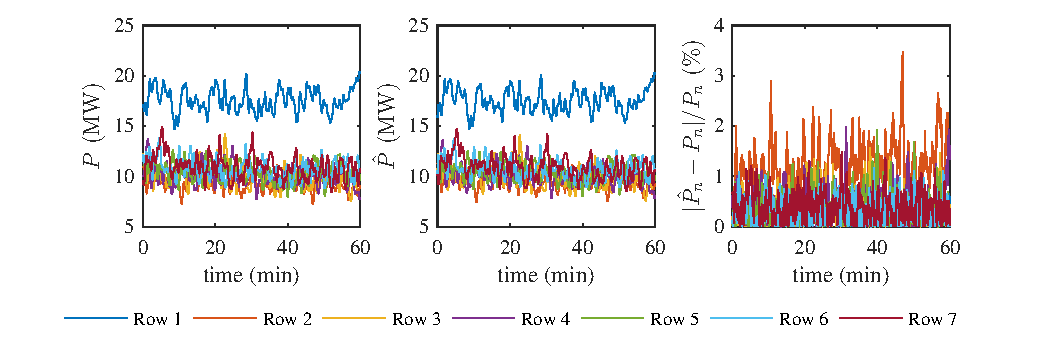
\includegraphics{./fig/r1-power.pdf}
\caption{Power generation of wind farm rows in LES (left) and the EnKF (center), as well as the instantaneous relative error of the wake model estimation for each row (right).}
\label{fig:r1-power}
\end{figure}

To examine the error in power estimation, we use the average relative estimation error measure $\frac{1}{T}\int_0^T |\hat{P}_n(t) - P_n(t)|/P_n(t) \, dt$ for each row, where $P_n(t)$ is the measured power in LES and $\hat{P}_n(t)$ is the estimated power. Table~\ref{tab:P_error} shows the average relative estimation error for all initial conditions. Instantaneous plots of the measured power from LES, the estimated power, and the relative error by row are shown in Figure~\ref{fig:r1-power}. Taken together, these results demonstrate that the instantaneous relative error does not exceed 4\% and the average relative estimation error is always less than 1.25\%.

\begin{figure}
\centering
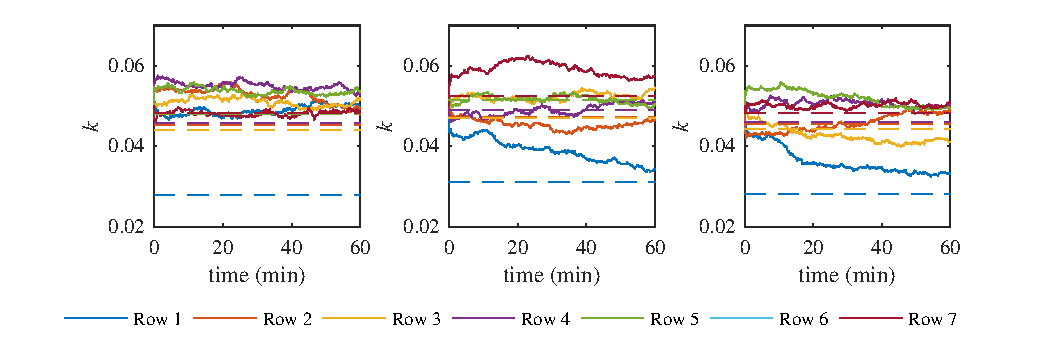
\includegraphics{./fig/k.pdf}
\caption{Comparison of wake expansion coefficients by row as calculated using EnKF (\full) and \textit{ex post facto} best fit of mean power generation using the wake model (\broken). Each panel shows a different initial condition. Two of the three panels capture the substantial difference between the wake expansion rates of the first row and subsequent rows.}
\label{fig:k}
\end{figure}


The estimated values of the wake expansion coefficients are shown in Figure~\ref{fig:k}. For each initial condition, the wake expansion coefficients are compared to a best-fit estimate of these coefficients from the average power of each row over the entire validation window. This best-fit is performed after the simulation and assumes a constant wake expansion rate for each turbine row for the entire window. For each initial condition, these best-fit coefficients demonstrate that the wake expansion rate is lower $k_1 \approx 0.03$ for the first row than subsequent rows $k_n \approx 0.05$. For the last two initial conditions, we see that the estimated wake expansion coefficients approach the distribution of wake expansion coefficients expected from the best fit. The first initial condition, however, does not approach the expected distribution, and more exploration is needed to study this case.


The wake model's streamwise velocity field $u(x,t)$ defined in~\eqref{eq:u} is compared to the LES velocity field $\tilde{u}(x,y,z_h,t)$ at the height of the turbine rotor $z_h$. In order to compare the modeled streamwise velocity along each turbine row, the row-averaged LES velocity field is computed using
\begin{equation}
\label{eq:u_tilde_avg}
\langle \tilde{u} \rangle(x,t) = \frac{1}{DM}\int_0^{L_y} \left[\sum_{m=1}^M H\left(\frac{D}{2}-|y-y_m|\right) \right] \tilde{u}(x,y,z_h,t) \, dy,
\end{equation}
where $H(y)$ is the Heaviside function and $y_m$ is the location of the $m$-th column of turbines. Figure~\ref{fig:u} compares a modeled streamwise velocity field using the EnKF $u(x,t)$ to a row-averaged streamwise velocity profile from LES $\langle \tilde{u} \rangle(x,t)$. This velocity field comparison demonstrates good correspondence between the measured and estimated velocity field near the location of each turbine and captures the changing wake expansion rates and advection of the velocity deficits. As expected, the errors increase downstream of each turbine where measurements are not available.

\begin{figure}[t!]
\centering
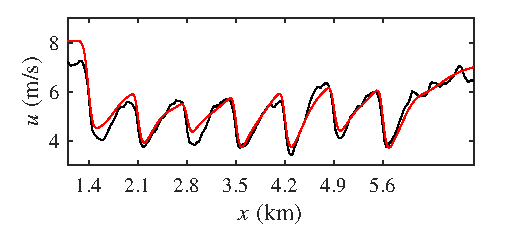
\includegraphics[width=0.65\textwidth]{./fig/u.pdf}
\caption{Instantaneous row-averaged velocity profile from LES (\full), as defined in~\eqref{eq:u_tilde_avg} and the EnKF wake model estimate ({\color{red}\full}), as defined in~\eqref{eq:u} and~\eqref{eq:enkf_final}. Each tick mark denotes a turbine row location.}
\label{fig:u}
\end{figure}

\section{Conclusions}
\label{sec:estimation-conclusons}
Sensing and estimation is vital for providing effective control through closed-loop feedback. In this chapter, we present two methods for providing error correction using measures of power within the wind farm. The first approach is simple to implement, but does not provide state and parameter correction. The second approach uses an EnKF to provide online state and parameter estimation in a computationally efficient manner. The addition of the EnKF provides a more practical approach for estimating wake model parameters and correcting wake model states because parameters do not have to be fit prior to initiation of the control.





